\subsection{Why use web corpora?}

\begin{frame}
  {Why corpora from the web?}

  \begin{itemize}
  \item \alert{Size}: alleviates data sparseness problems with rare phenomena
  \item \alert{Content}: registers not found in traditional corpora\\ (forum discussions, blogs, fan-fiction etc.)
  \item \alert{Replicability}: research with static corpus\\
    vs.\ research based on search engine results
  \item \alert{Availability}: data can be locally processed with preferred tools.
  \item \alert{Cost}: (virtually) free
  \end{itemize}
\end{frame}


\begin{frame}
  {Some potential drawbacks of web corpora}

  \begin{itemize}
  \item \alert{Noise}: from properties of web documents\\
    and from imperfect processing
  \item \alert{Meta data} (of the kind linguists are interested in):\\
    not encoded in web documents in a reliable way
  %   \begin{itemize}
%     \item no stratification by registers and/or text types
%     \item either manual classification (unrealistic for very large corpora)
%     \item or automatic classification, based on easy-to-compute features
%     \end{itemize}
  \end{itemize}
\end{frame}


\subsection{Web corpus construction: Overview}

\begin{frame}{Web corpus construction: workflow}

\scalebox{.7}{
  \begin{tabular}{c}
    \fbox{\alert<2->{Data collection}}\\[.6ex]
$\Downarrow$\\[.6ex]
    \fbox{Removal of markup, scripts etc. }\\[.6ex]
$\Downarrow$\\[.6ex]
    \fbox{\alert<2->{Detection/removal of ``boilerplate''}}\\[.6ex]
$\Downarrow$\\[.6ex]
    \fbox{\alert<2->{Detection/removal of ``non-texts''}}\\[.6ex]
$\Downarrow$\\[.6ex]
    \fbox{\alert<2->{Detection/removal of (near-) duplicates}}\\[.6ex]
$\Downarrow$\\[.6ex]
    \fbox{\alert<2->{Linguistic post-processing}}
  \end{tabular}
}

\vspace{.5cm}
 \onslide<2->{
These steps involve design decisions\\
which affect the properties of the final corpus.}
\end{frame}


\begin{frame}{Workflow II}
  \begin{columns}
    \begin{column}{5cm}
    \scalebox{.7}{
\begin{tabular}{c}

\fbox{\alert<1>{Data collection}}\\[.6ex]
$\Downarrow$\\[.6ex]
    \fbox{Removal of markup, scripts etc. }\\[.6ex]
$\Downarrow$\\[.6ex]
    \fbox{\alert<2>{Detection/removal of ``boilerplate''}}\\[.6ex]
$\Downarrow$\\[.6ex]
    \fbox{\alert<3>{Detection/removal of ``non-texts''}}\\[.6ex]
$\Downarrow$\\[.6ex]
    \fbox{\alert<4>{Detection/removal of (near-) duplicates}}\\[.6ex]
$\Downarrow$\\[.6ex]
    \fbox{\alert<5->{Linguistic post-processing}}
\end{tabular}
}
    \end{column}

    \begin{column}{5cm}
      \begin{itemize}
      \item Which sampling procedure/crawling strategy?
      \item<2-> What should count as ``boilerplate''?
      \item<3-> Which documents contribute ``good text''?
      \item<4-> Which amount of duplication is acceptable?
      \item<5-> How do we treat non-standard orthography, spelling errors, non-words etc.?
      \end{itemize}
    \end{column}
  \end{columns}
\end{frame}



%\subsection{Data collection}
%
%%\subsection{The Web (Graph)}
%
%\begin{frame}
%  {Links}
%  \begin{itemize}
%    \item The web consists of pages and links between them.
%    \item Each page has an \alert{in-degree} (no.\ of links to that page),
%    \item and an \alert{out-degree} (no.\ of links on that page).
%  %  \item The in-degree of pages is distributed by a \alert{power law}\\
%  %    ($\frac{1}{a^{2.1}}$ according to \citealp[][426]{Manning-ea2009}.)
%    \item Pages with a higher in-degree are easier to find, but not necessarily the more interesting ones for corpus construction.
%  \end{itemize}
%\end{frame}
%
%\begin{frame}
%  {The structure of the web}
%  \begin{center}
%    
\includegraphics[width=6cm]{graphicswcc/bowtie}\\
%    
%    \vspace{0.5cm}
%    \footnotesize\cite[427]{Manning-ea2009}\\
%    Contrary to common intuition, \citealp{Broder-ea00} found that the IN, OUT, SCC, and TENDRIL components are not extremely different in size.\\
%    A more detailed report on the sizes: \cite{Serrano-ea2007}.
%  \end{center}
%\end{frame}
%
%\begin{frame}
%  {Inaccessible web content (deep web)}
%  \begin{itemize}
%    \item explicitly \alert{hidden} from spiders\\
%      (Robots Exclusion, intentional fooling\slash spoofing)
%    \item requiring \alert{login}\\
%      (social networks, some forums, intranet gateways)
%    \item \alert{in-degree$=0$}
%    \item \graw{in-degree$>0$, but \alert{too far away} from any seed URL\\
%    (which are mostly search-engine indexed pages;\\
%  depends on crawling strategy)}
%  \end{itemize}
%\end{frame}
%
%\begin{frame}
%  {Static and dynamic web content}
%  \begin{itemize}
%    \item By definition, \alert{static web content} is any page which is\\
%      not generated by a database\slash content generation system,\\
%      but edited manually.
%    \item Today, most content is \alert{dynamic} (CMS, blogs, etc.),\\
%      and the static\slash dynamic distinction should not play\\
%      a great role in crawling for corpus construction.
%    \item The problem is rather the separation of (static or dynamic) \alert{linguistically relevant} from \alert{irrelevant} content\\
%      (time tables, product listings, etc.).
%  \end{itemize}
%\end{frame}
%
%\begin{frame}
%  {Top-level domains and national dialects}
%  \begin{itemize}
%    \item It is common practice to crawl national TLDs for content\\
%      in the corresponding national language.
%    \item \cite{Cook-Hirst2012} conclude that the TLDs for \texttt{.ca}\\
%      and \texttt{.uk} indeed \alert{represent national variants} of English.
%   % \item Methods used: \alert{keyword} comparison with existing corpora \citep{Kilgarriff2009}, \alert{spelling variants}.
%    \item Problems with TLD crawls:
%      \begin{itemize}
%	\item In some countries, \texttt{.com} has a high prestige:\\
%	  \url{http://elpais.com}, \url{http://www.lavanguardia.com/}, \url{http://www.marca.com/}
%	\item TLDs of countries with more than one official language\\
%	  (\eg, Indonesia, Spain) yield relatively fewer results\\
%	  in the target language.
%      \end{itemize}
%   \end{itemize}
%\end{frame}
%
%
%
%\begin{frame}{Breadth-first crawling}
%
%Common practice (e.\,g.\ WaCky, COW): follow \textbf{all} links on a page\\[2ex]
%
%Pro:
%
%  \begin{itemize}
%  \item effective: yields lots of data whithin a short time
%  \item open source software available 
%  \end{itemize}
%
%Con:
%
%\begin{itemize}
%\item very susceptible to page rank: no uniform random sample
%\item unknown sampling bias
%\end{itemize}
%  
%\end{frame}
%
%
%\begin{frame}
%  {Alternative: Random walks}
%
%Yet not used for web corpora: follow \textbf{one} link on a page
%
%Pro:
%
%\begin{itemize}
%\item known sampling bias: can be corrected for
%\item uniform random sample of web documents
%\end{itemize}
%
%Con:
%
%\begin{itemize}
%\item much less effective than BF
%\item probably not suitable for giga-token corpora
%\end{itemize}
%
%\end{frame}





\subsection{Boilerplate detection}

\begin{frame}
  {Boilerplate detection}

Boilerplate is text accompanying the main text on a web page:

\begin{itemize}
\item navigation bars
\item banners
\item advertisements
\item other layout elements 
\item copyright notes
\end{itemize}

\pause

Boilerplate is typically not text produced by person on a particular occasion, but rather

\begin{itemize}
\item generated by content management systems
\item similar or identical on many web pages of the same website
\item similar or identical across web sites 
\end{itemize}
\end{frame}


\begin{frame}
  {Why detect boilerplate?}

Boilerplate elements bias the frequency of linguistic items in the final corpus.

\begin{itemize}
\item One of the most frequent tokens in an experimental German web corpus: \textit{mehr} `more', as in \textit{read more\ldots}\\[1ex] \pause
\item One of the most frequent sentences in an experimental English web corpus: \textit{You are not allowed to post new content in the forum.}
\end{itemize}
\end{frame}


\begin{frame}
  {Text}
  \begin{center}
    
\includegraphics[width=8cm]{graphicswcc/webseite}
  \end{center}
\end{frame}

\begin{frame}
  {Text (II)}
  \begin{center}
    
\includegraphics[width=8cm]{graphicswcc/webseite2}
  \end{center}
\end{frame}

\begin{frame}
  {Text (III)}
  \begin{center}
    \includegraphics[width=8cm]{graphicswcc/webseite3}
  \end{center}
\end{frame}




\begin{frame}
  {What should count as boilerplate? }
  \begin{center}
    
\includegraphics[width=8cm]{graphicswcc/webseite}
  \end{center}
\end{frame}

\begin{frame}
  {What should count as boilerplate? (II)}
  \begin{center}
    \includegraphics[width=8cm]{graphicswcc/webseite-b}
  \end{center}
\end{frame}


\begin{frame}
  {What should count as boilerplate? (III)}
  \begin{center}
    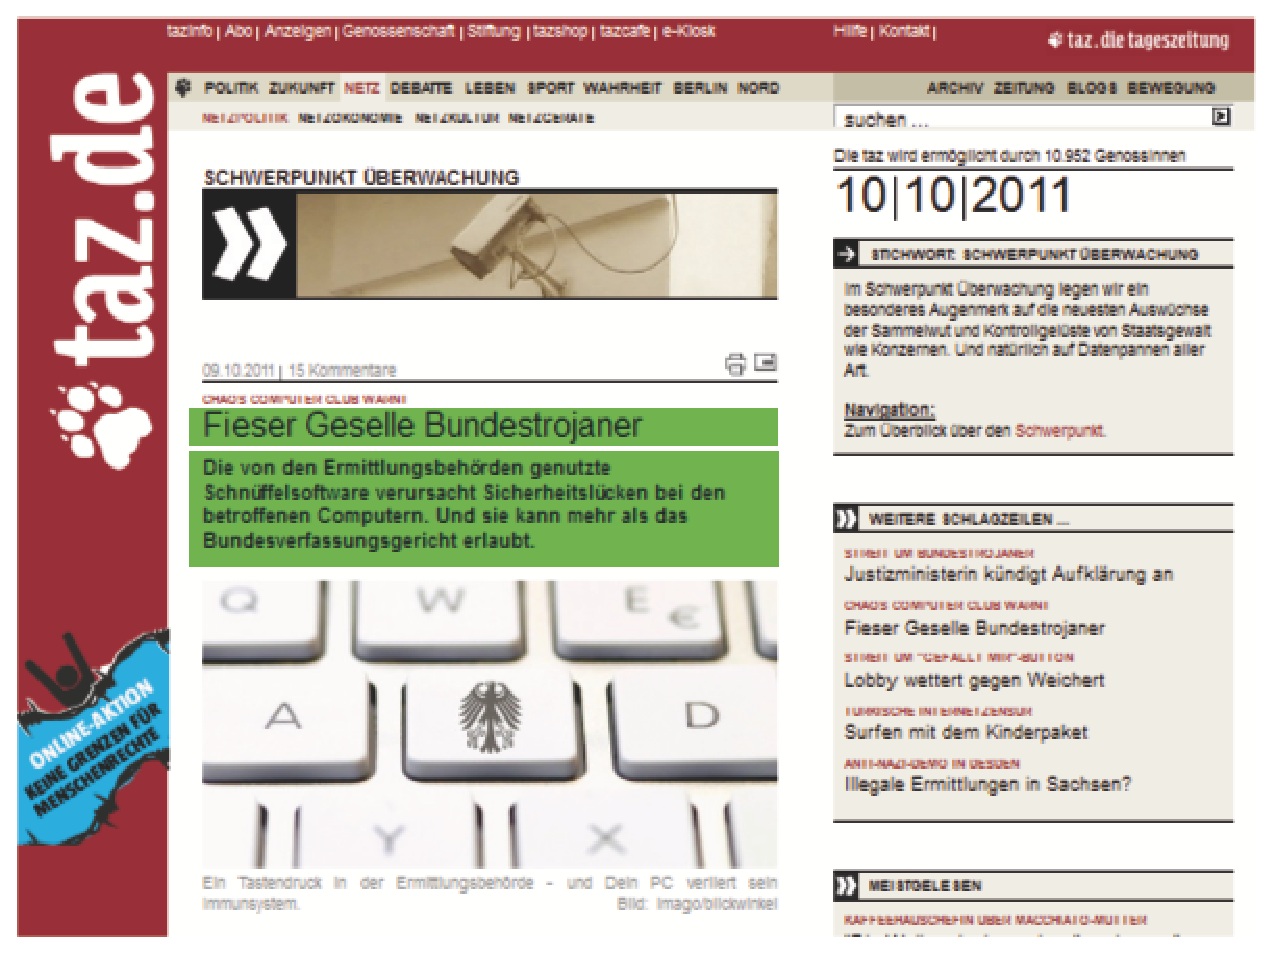
\includegraphics[width=8cm]{graphicswcc/webseite-c}
  \end{center}
\end{frame}



\begin{frame}
  {What should count as boilerplate? (IV)}
  \begin{center}
    \includegraphics[width=8cm]{graphicswcc/webseite-d}
  \end{center}
\end{frame}


\begin{frame}
  {What should count as boilerplate? (V)}
  \begin{center}
    \includegraphics[width=8cm]{graphicswcc/webseite-e}
  \end{center}
\end{frame}



\begin{frame}
  {What should count as boilerplate?(VI)}
  \begin{center}
    \includegraphics[width=8cm]{graphicswcc/webseite3}
  \end{center}
\end{frame}


\begin{frame}
  {What should count as boilerplate? (VII)}
  \begin{center}
    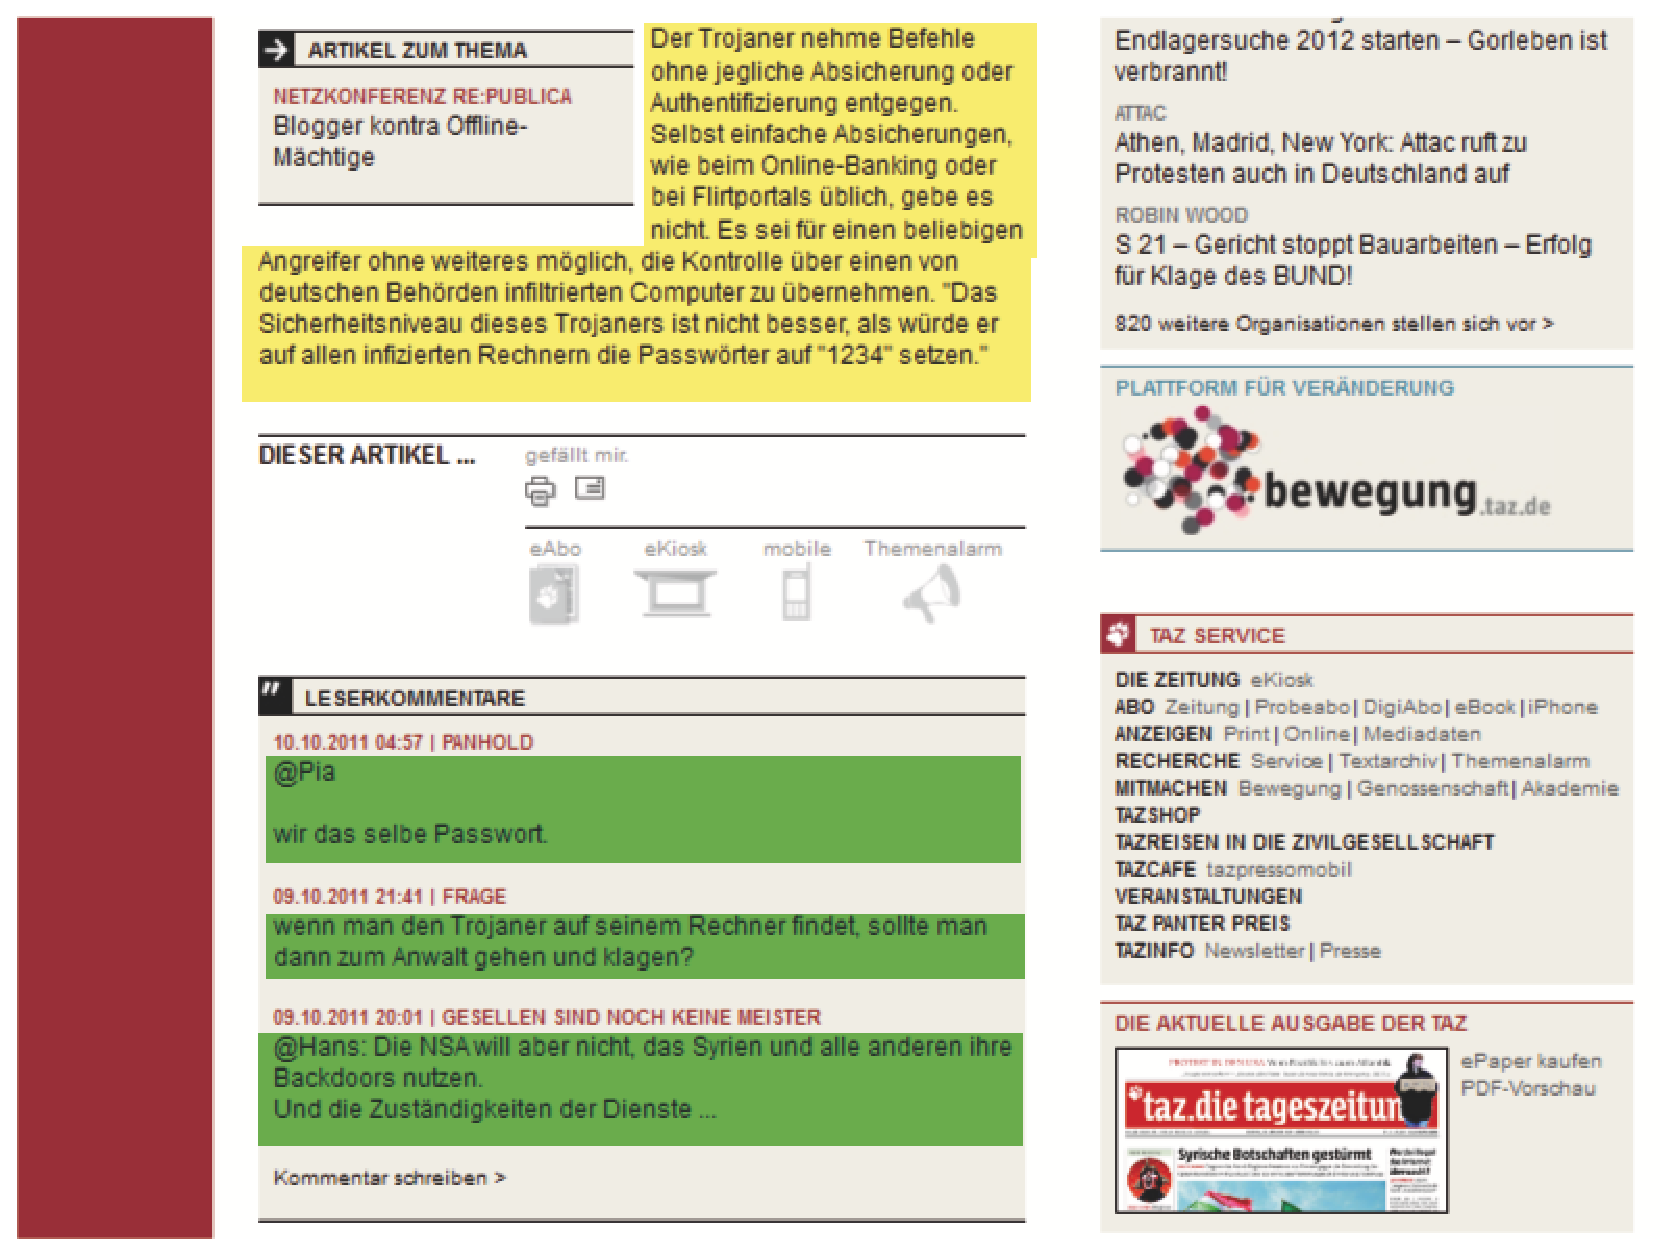
\includegraphics[width=8cm]{graphicswcc/webseite3-b}
  \end{center}
\end{frame}


\begin{frame}
  {What should count as boilerplate? (VIII)}
  \begin{center}
    \includegraphics[width=8cm]{graphicswcc/webseite3-c}
  \end{center}
\end{frame}


\begin{frame}
  {What should count as boilerplate?  (IX)}
  \begin{center}
    \includegraphics[width=8cm]{graphicswcc/webseite3-d}
  \end{center}
\end{frame}


\begin{frame}
  {What should count as boilerplate? (X)}
  \begin{center}
    \includegraphics[width=8cm]{graphicswcc/webseite3-e}
  \end{center}
\end{frame}


\begin{frame}
{Automatic detection of boilerplate}

Boilerplate must be detected automatically.\\[2ex] %, given   Typical web corpora contain millions of documents:

Machine learning techniques:
\begin{itemize}
\item Manually annotate a number of paragraphs: boilerplate yes/no
\item Calculate a number of features from each paragraph
  \begin{itemize}
  \item e.\,g., number of text characters, number of HTML tags, position in HTML-document
  \end{itemize}
\item Train a classifier to reproduce the human's decisions 
  \begin{itemize}
  \item we use an artificial neural network (multilayer perceptron)
  \end{itemize}
\end{itemize}
\end{frame}


% \begin{frame}
%   {Overview of the boilerplate removal scene}
%   \begin{itemize}
%     \item Most prominently, the \alert{CLEANEVAL} competition \citep{Baroni-ea2008} produced a variety of efforts in boilerplate removal and document structure recognition:
%       \begin{itemize}
% 	\item \cite{Bauer-ea2007}, \cite{Evert2007}, \cite{Weizheng-Abou2007}, \cite{Girardi2007}, \cite{Hoffman-Weerkamp2007}, \cite{Issac2007}, \cite{Marek-ea2007}, \cite{Saralegi-Leturia2007}
%       \end{itemize}
%     \item Furthermore, the WaCky corpora have undergone some boilerplate removal method \citep{Baroni-ea2009}.
%     \item Claiming to have achieved a very high accuracy: \cite{Spousta2008}, based on \cite{Marek-ea2007}.
%     \item You can also check out JustText at \url{http://nlp.fi.muni.cz/projekty/justext/} online, based on \cite{Pomikalek2011}.
%   \end{itemize}
% \end{frame}


\begin{frame}
{Automatic detection of boilerplate (II)}

Automatic detection is not perfect:

\begin{itemize}
\item some boilerplate will not be discovered (recall $<1$)
\item some paragraphs will be mistakenly classified as boilerplate (precision $<1$)
\end{itemize}

Keep this in mind when working with web corpora,\\
and double check any implausible frequency figures.
  
\end{frame}



\begin{frame}{Boilerplate: removal vs.\ flagging}
  
``Classic'' approach (e.\,g., WaCky, COW2012): remove boilerplate.

  \begin{itemize}
  \item Alternative: do not remove, but flag\\
    (possibly with a confidence score)
    \item \alert{Pro} -- User do not have to rely on:
      \begin{itemize}
      \item the corpus designer's definition of boilerplate
      \item the performance of an automatic classifier
      \end{itemize}
\pause
    \item \alert{Con}:
      \begin{itemize}
      \item increase in corpus size
%      \item depending on querying architecture: 
      \end{itemize}
  \end{itemize}
\end{frame}


\subsection{Document filtering}


\begin{frame}
{Document filtering}

Ideally, the final corpus should contain only ``good'' documents.

``Good'':

\begin{itemize}
\item only documents in the target language
\item documents containing predominantly text\\
  (i.\,e., coherent and connected text)
\end{itemize}

\pause

This excludes certain document types:

\begin{itemize}
\item lists (e.\,g.\ company names, vocabulary items)
\item tag clouds
\item etc.
\end{itemize}

\end{frame}



\begin{frame}{Example: a ``good'' document}
  
  \begin{center}
     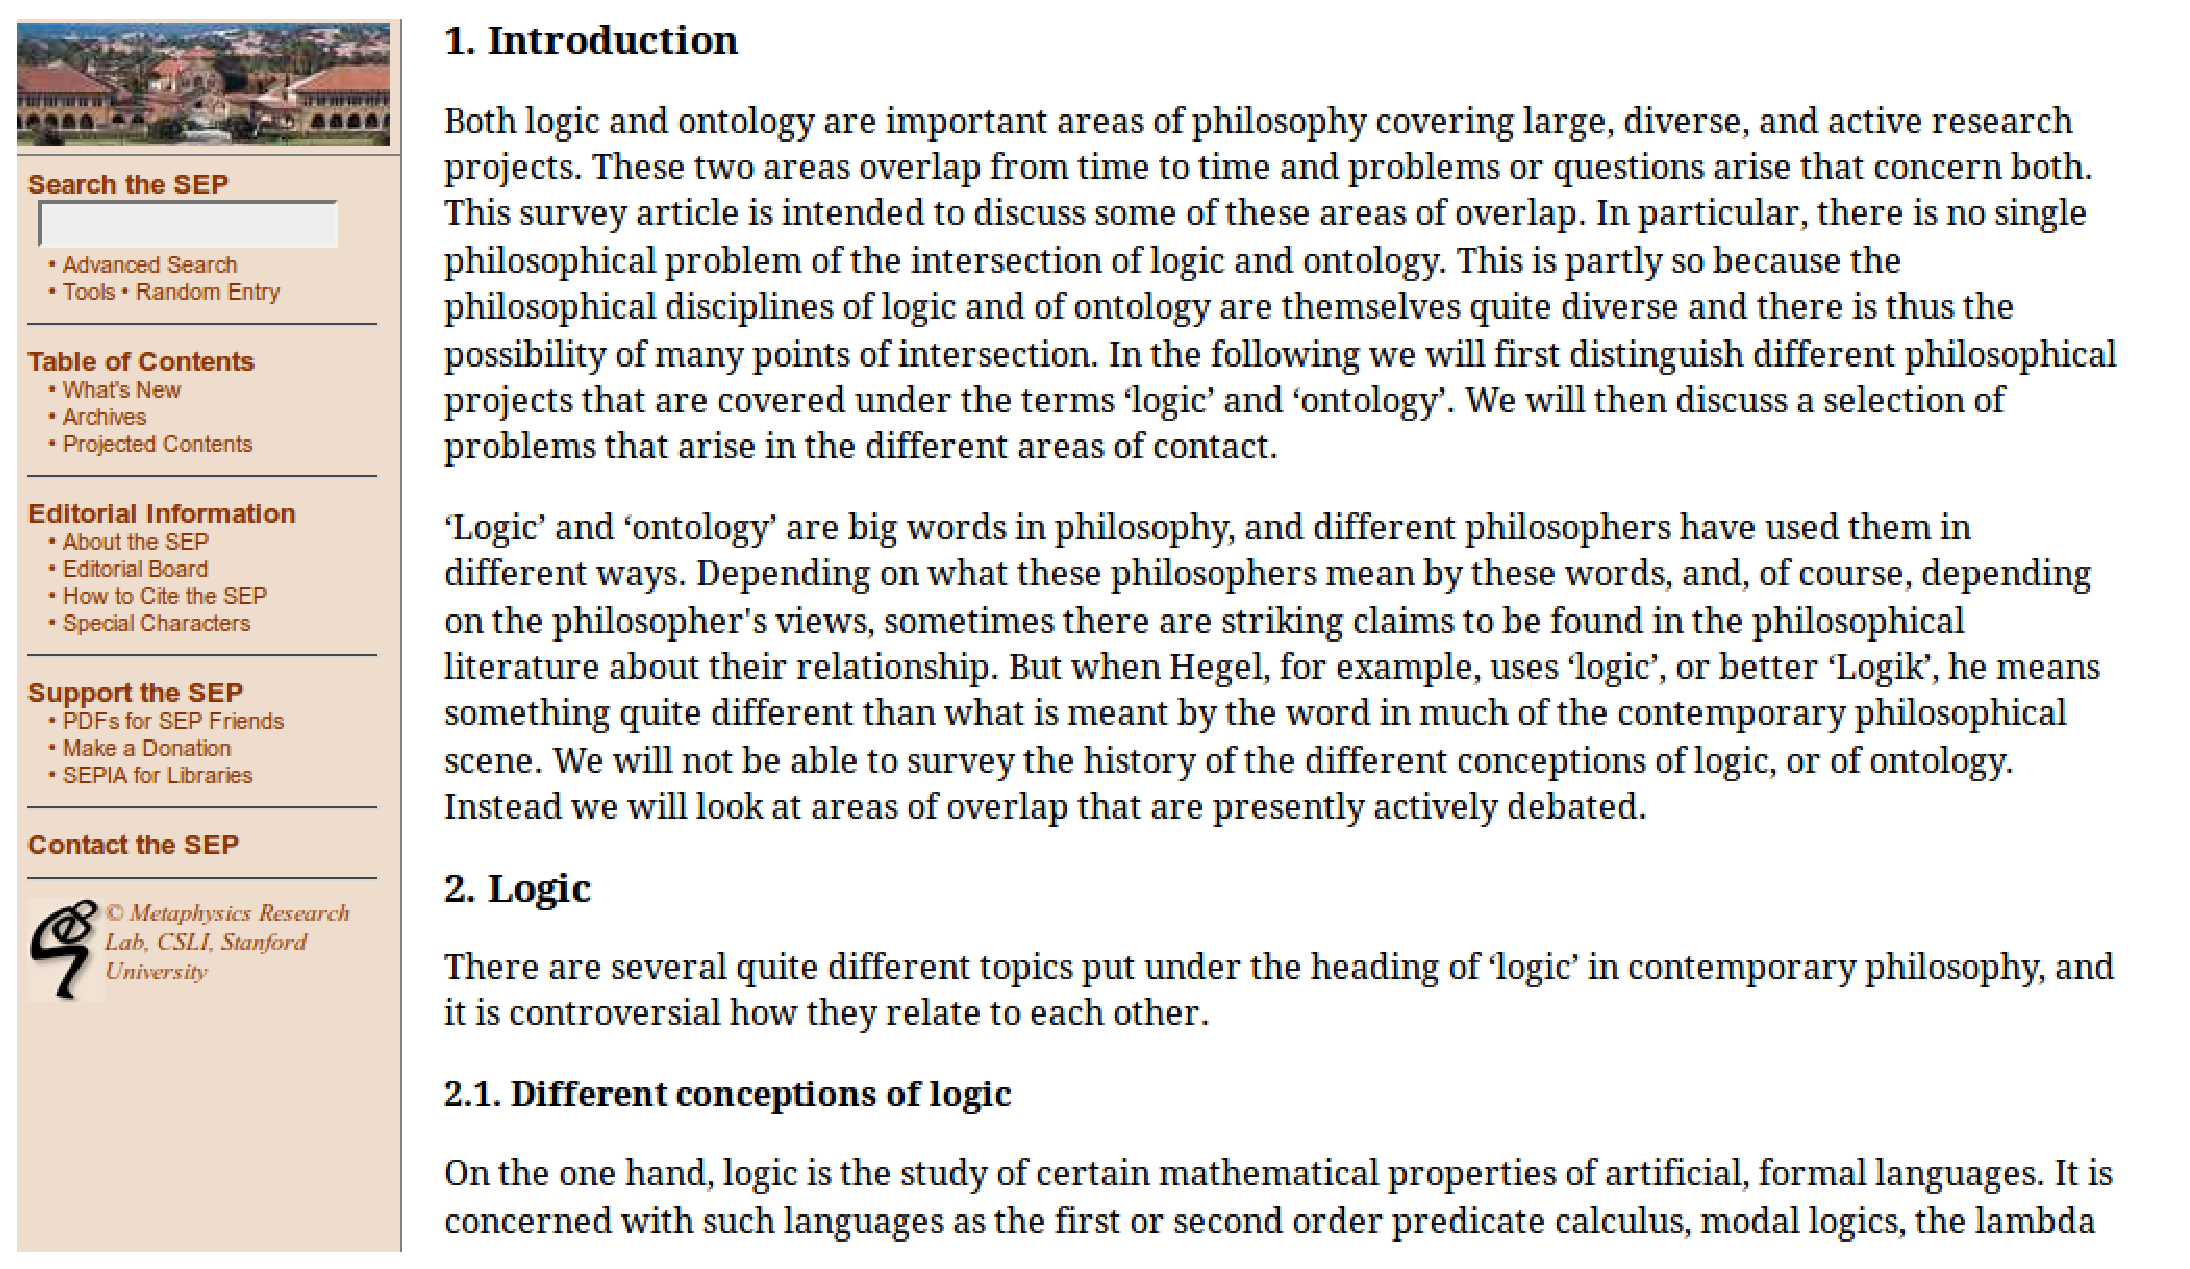
\includegraphics[width=8cm]{graphicswcc/good}
  \end{center}

\end{frame}



\begin{frame}
{Distinguishing the ``good'' from the ``bad'' (I)}  

\begin{itemize}
\item Classification has to be performed automatically
\item ML algorithms usually need manually annotated training data 
\item But: the decision is difficult even for humans and arbitrary to some extent
\end{itemize}
\pause

Experiment: 3 raters, 1000 random documents from German web corpus, using 5-point scale:

 \begin{itemize}
	\item $-2,-1$: document \alert{should not} be in the corpus 
	\item $1, 2$: document \alert{should} be in the corpus 
	\item $0$: undecided\slash document \alert{might or might not} be in the corpus
 \end{itemize}

 \end{frame}

\begin{frame}
{Distinguishing the ``good'' from the ``bad'' (II)}
Results (after training phase of rating of 100 documents together, with several hours of discussion of borderline cases):


  \begin{center}
\scalebox{.8}{
  \begin{tabular}{lrrr}
    \hline
    statistic & early 500 & late 500 & all 1,000 \\
    \hline
    \hline
    raw & 0.566 & 0.300 & \alert<2->{0.433} \\
    $\kappa$ (raw) & $0.397$ & $0.303$ & $0.367$ \\
    $ICC(C,1)$ & $0.756$ & $0.679$ & $\alert<2->{0.725}$ \\
    \hline
    raw ($r\geq0$) & 0.900 & 0.762 & \alert<2->{0.831} \\
    raw ($r\geq1$) & 0.820 & 0.674 & 0.747 \\
    $\kappa$ ($r\geq0$) & $0.673$ & $0.625$ & $\alert<2->{0.660}$ \\
    $\kappa$ ($r\geq1$) & $0.585$ & $0.555$ & $0.598$ \\
    $\kappa$ ($r\geq2$) & $0.546$ & $0.354$ & $0.498$ \\
    \hline
  \end{tabular}
}
  \end{center}

\end{frame}




\begin{frame}{``Good'' vs.\ ``bad'' documents: lists}

   \begin{center}
    \includegraphics[width=8cm]{graphicswcc/rezept}
  \end{center}

\end{frame}



\begin{frame}{``Good'' vs.\ ``bad'' documents: lists (II)}

   \begin{center}
    \includegraphics[width=11cm]{graphicswcc/kunststoff}
  \end{center}

\end{frame}


\begin{frame}{``Good'' vs.\ ``bad'' documents: lists (III)}

   \begin{center}
    
\includegraphics[width=8cm]{graphicswcc/spedition}
  \end{center}

\end{frame}


\begin{frame}
  {Acceptable results?}
  \begin{itemize}
    \item \alert{values below $0.68$ \citep{Krippendorff1980}}
    \item even considering criticism of Krippendorf's magic number\\
      \citep{Carletta1996,BayerlPaul2011}:\\
      \alert{uncomfortably low for ``gold standard''}
    \item more confusion on late data (lower overall quality)
    \item worse: disagreement between corpus designers
    \item acceptance at the threshold $\geq 0$:\\
      A: 78.4\%, R: 73.8\%, S: 84.9\%
  \end{itemize}
\end{frame}

%\subsection{Badness scores}

\begin{frame}
  {General method and idea}
  \begin{itemize}
    \item simple metric with known properties
    \item language-independent, unsupervised\ldots\\
      \alert{does not involve an obviously difficult design decision}
    \item strategy for cleansing: \alert{high recall for everyone},\\
      accept mediocre precision
    \item for retained documents: use as annotation in final corpus,\\
      \alert{allow corpus users to ``set'' precision}
  \end{itemize}
\end{frame}

\begin{frame}
  {Implementation}
  \begin{itemize}
    \item based on ``frequent\slash short word'' method\\
      in language identification \citep{Grefenstette1995}
    \item similar to WaCky \citep{Baroni-ea2009}\\
      but without manually compiled lists of function words
    \item totally unsupervised procedure for crawled data\\
      predominantly in a single language (TLD crawl):
      \begin{itemize}
	\item \alert{training}: get weighted mean and standard deviation\\
	  of relative frequencies of the most frequent words (``profile'')
	\item \alert{production}: calculate for the top $m$ of them\\
	  the ``standardized'' negative deviation for each document\\
	\item clamped and added up: the \alert{Badness score}
      \end{itemize}
  \end{itemize}
\end{frame}


\subsection{Duplication}


\begin{frame}
{Duplicate sentences in a corpus concordance}


Query: \texttt{made a donation}

\vspace{1cm}

   \begin{center}
     \alt<1>{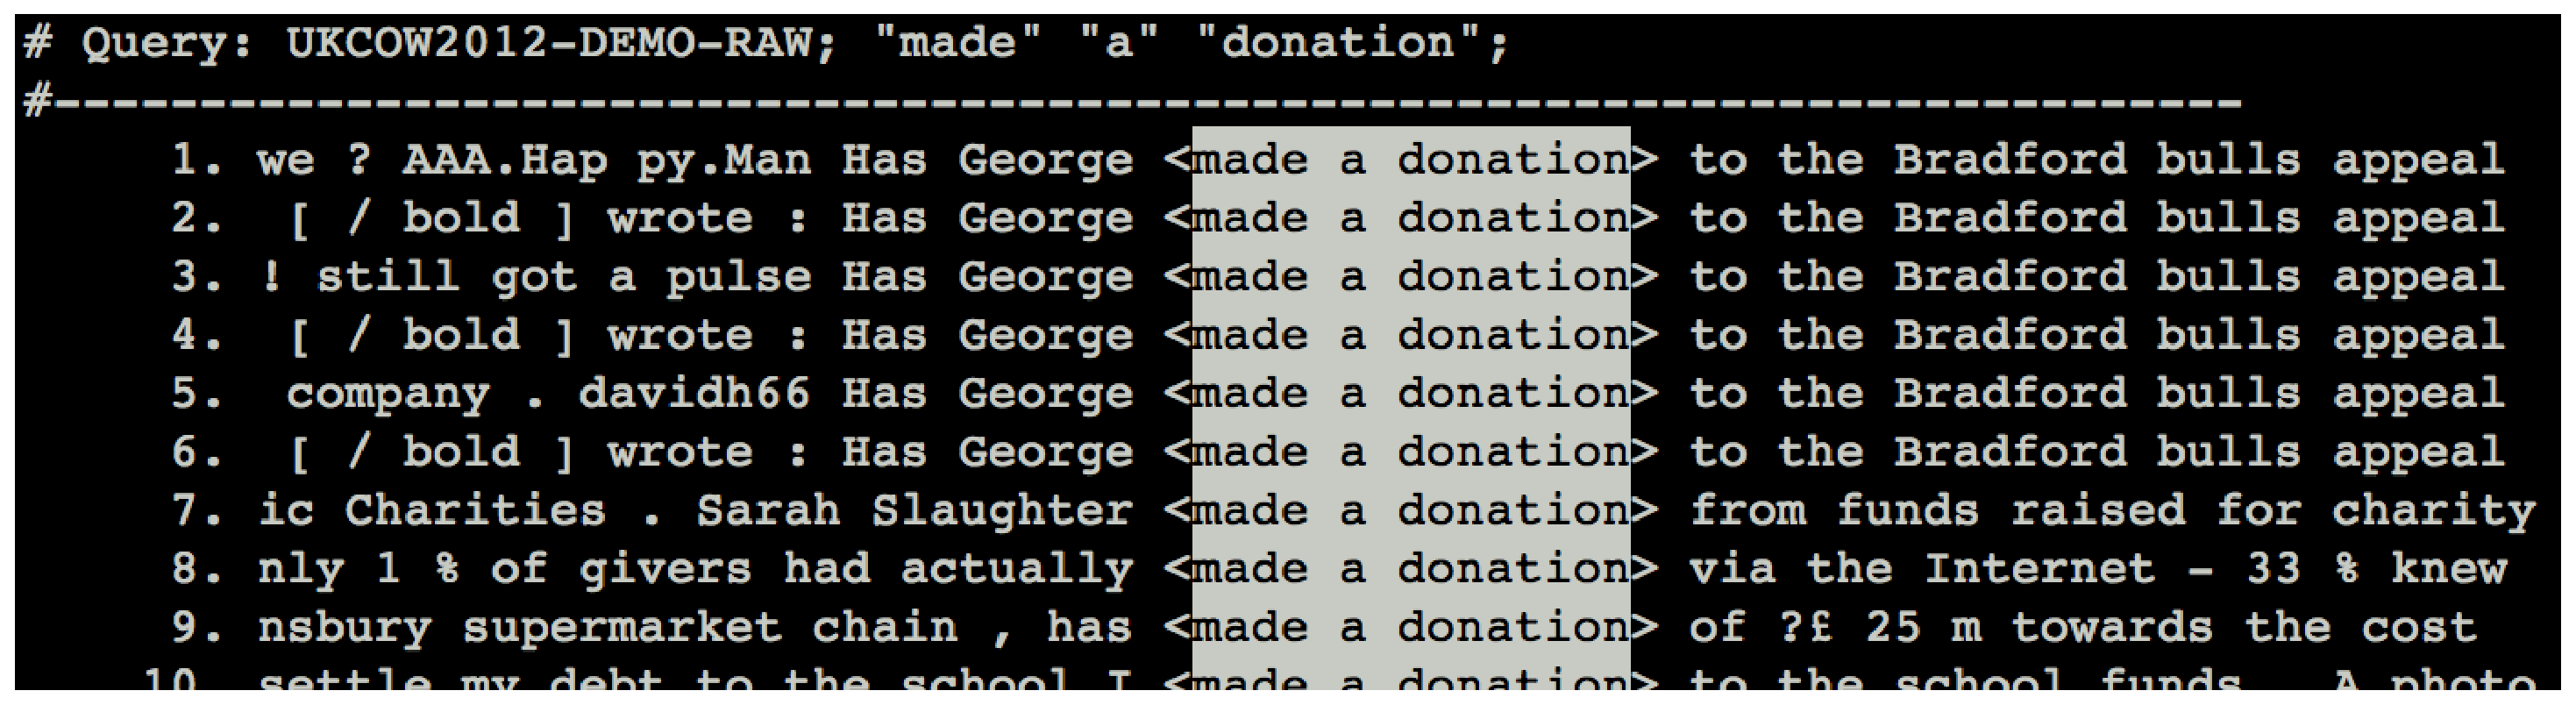
\includegraphics[width=10cm]{graphicswcc/donation}}{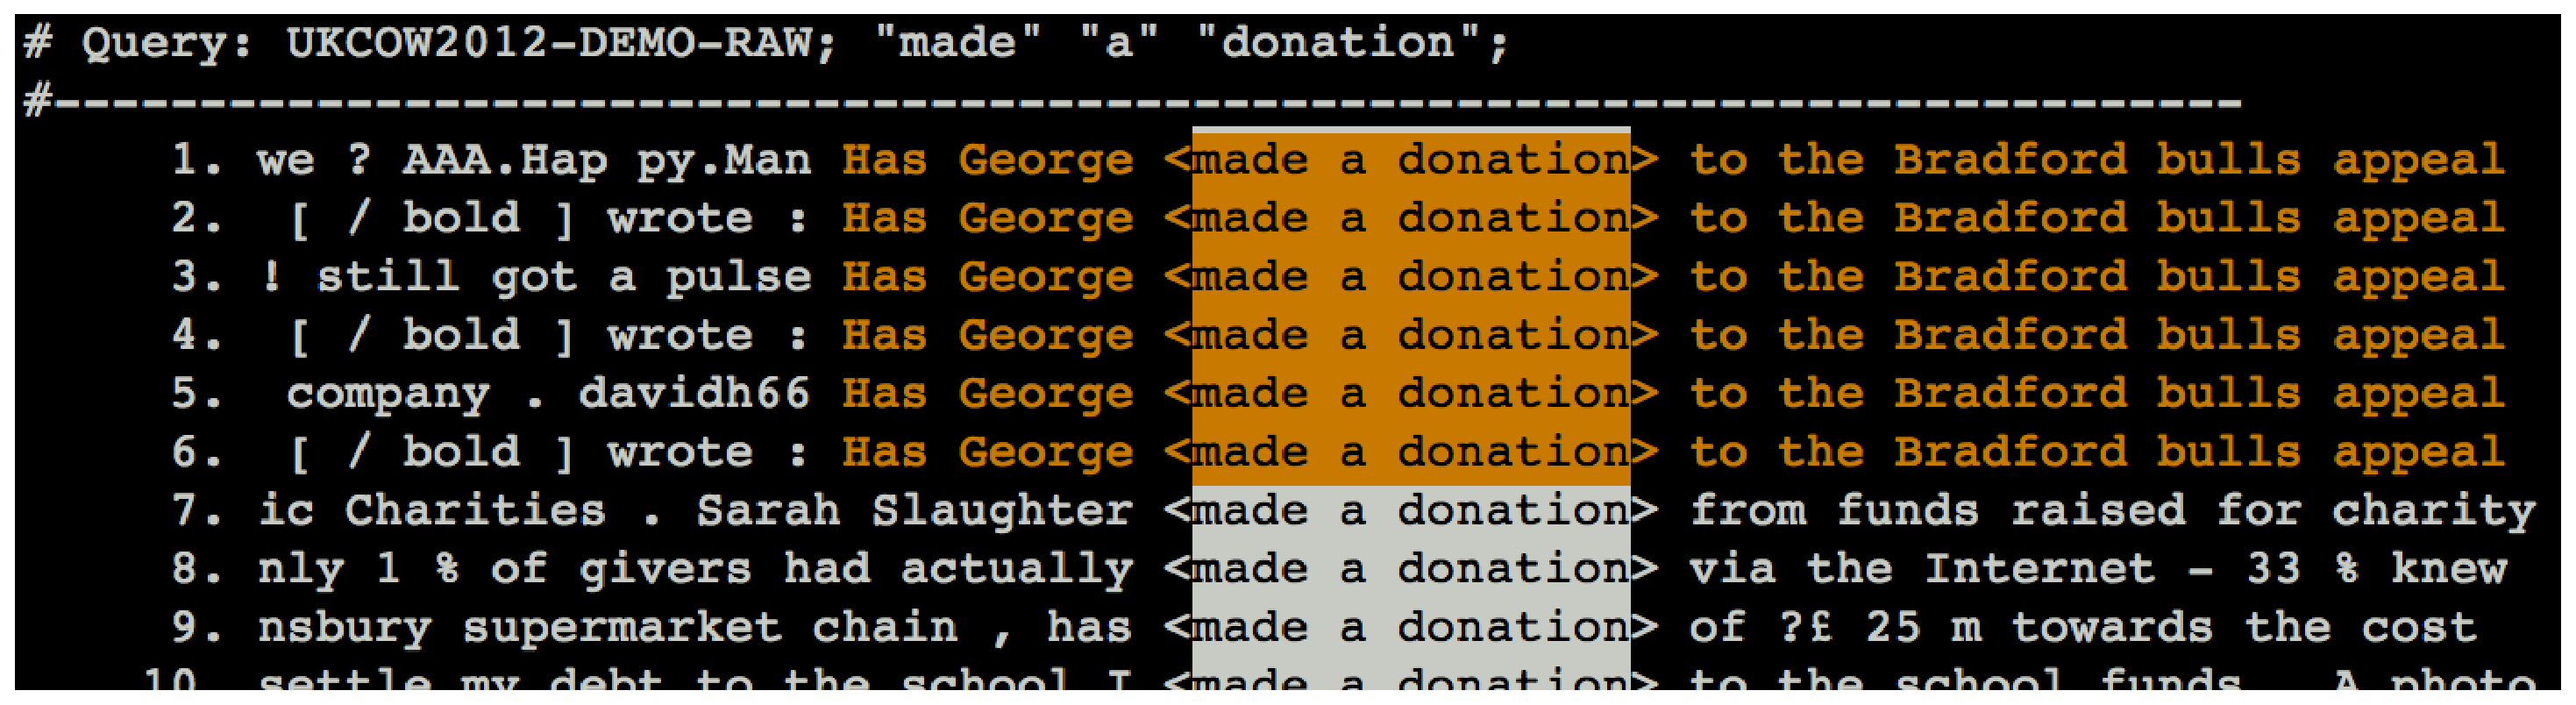
\includegraphics[width=10cm]{graphicswcc/donation2}}\\
   \end{center}  

\pause

\end{frame}



\begin{frame}
   \begin{center}
     
\includegraphics[width=10cm]{graphicswcc/argus2}\\
   \end{center}  
\end{frame}


 \begin{frame}

   \begin{center}
     
\includegraphics[width=8cm]{graphicswcc/george1col2}\\
   \end{center}
\pause
  \begin{center}
     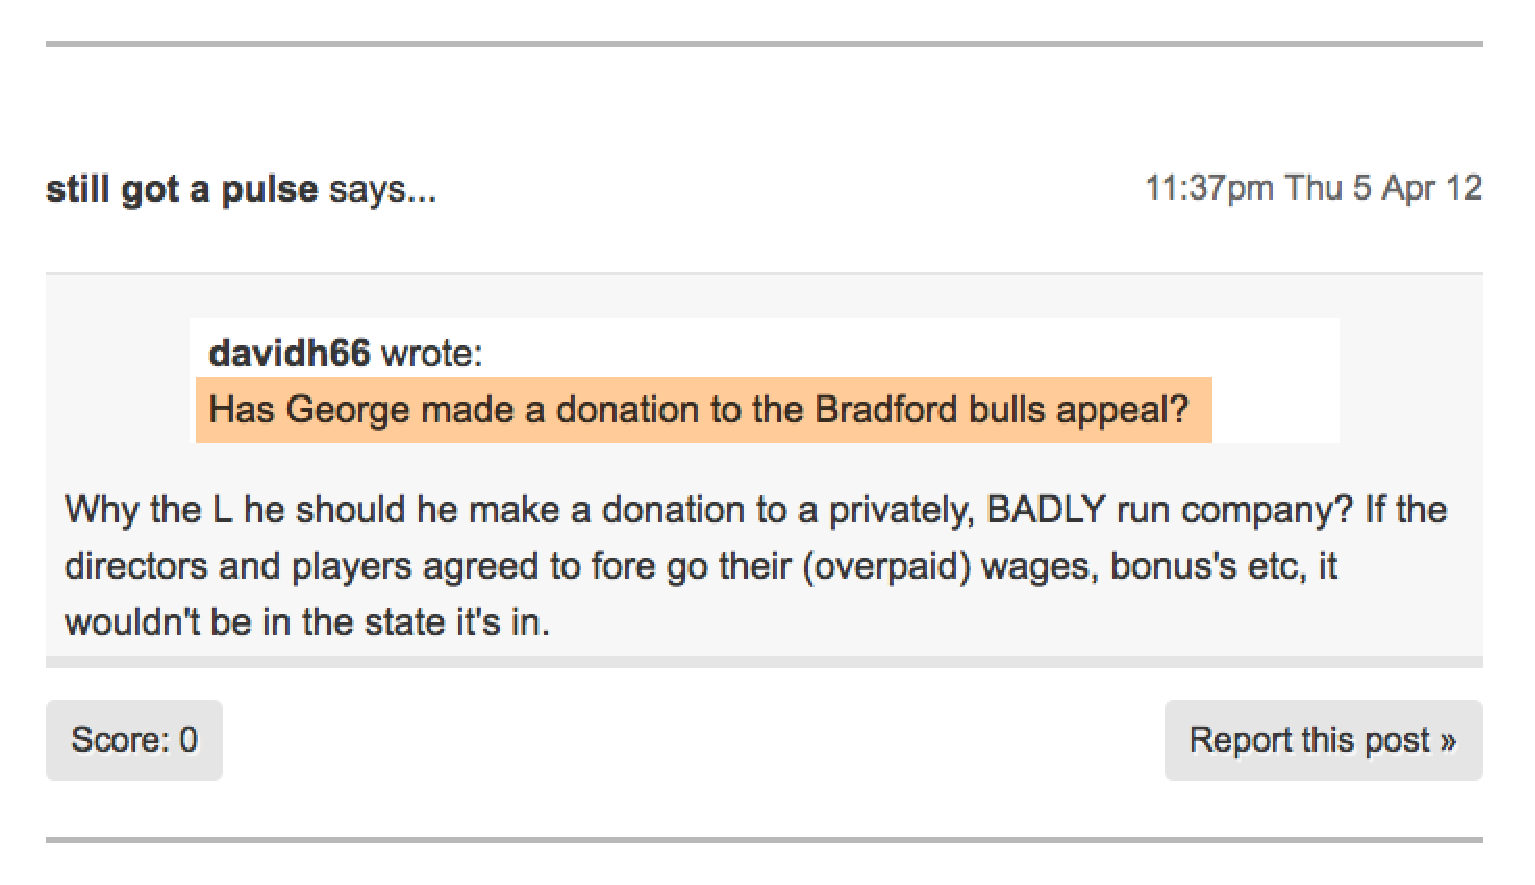
\includegraphics[width=8cm]{graphicswcc/george2col2}\\
   \end{center}

 \end{frame}


 \begin{frame}
   \begin{center}
     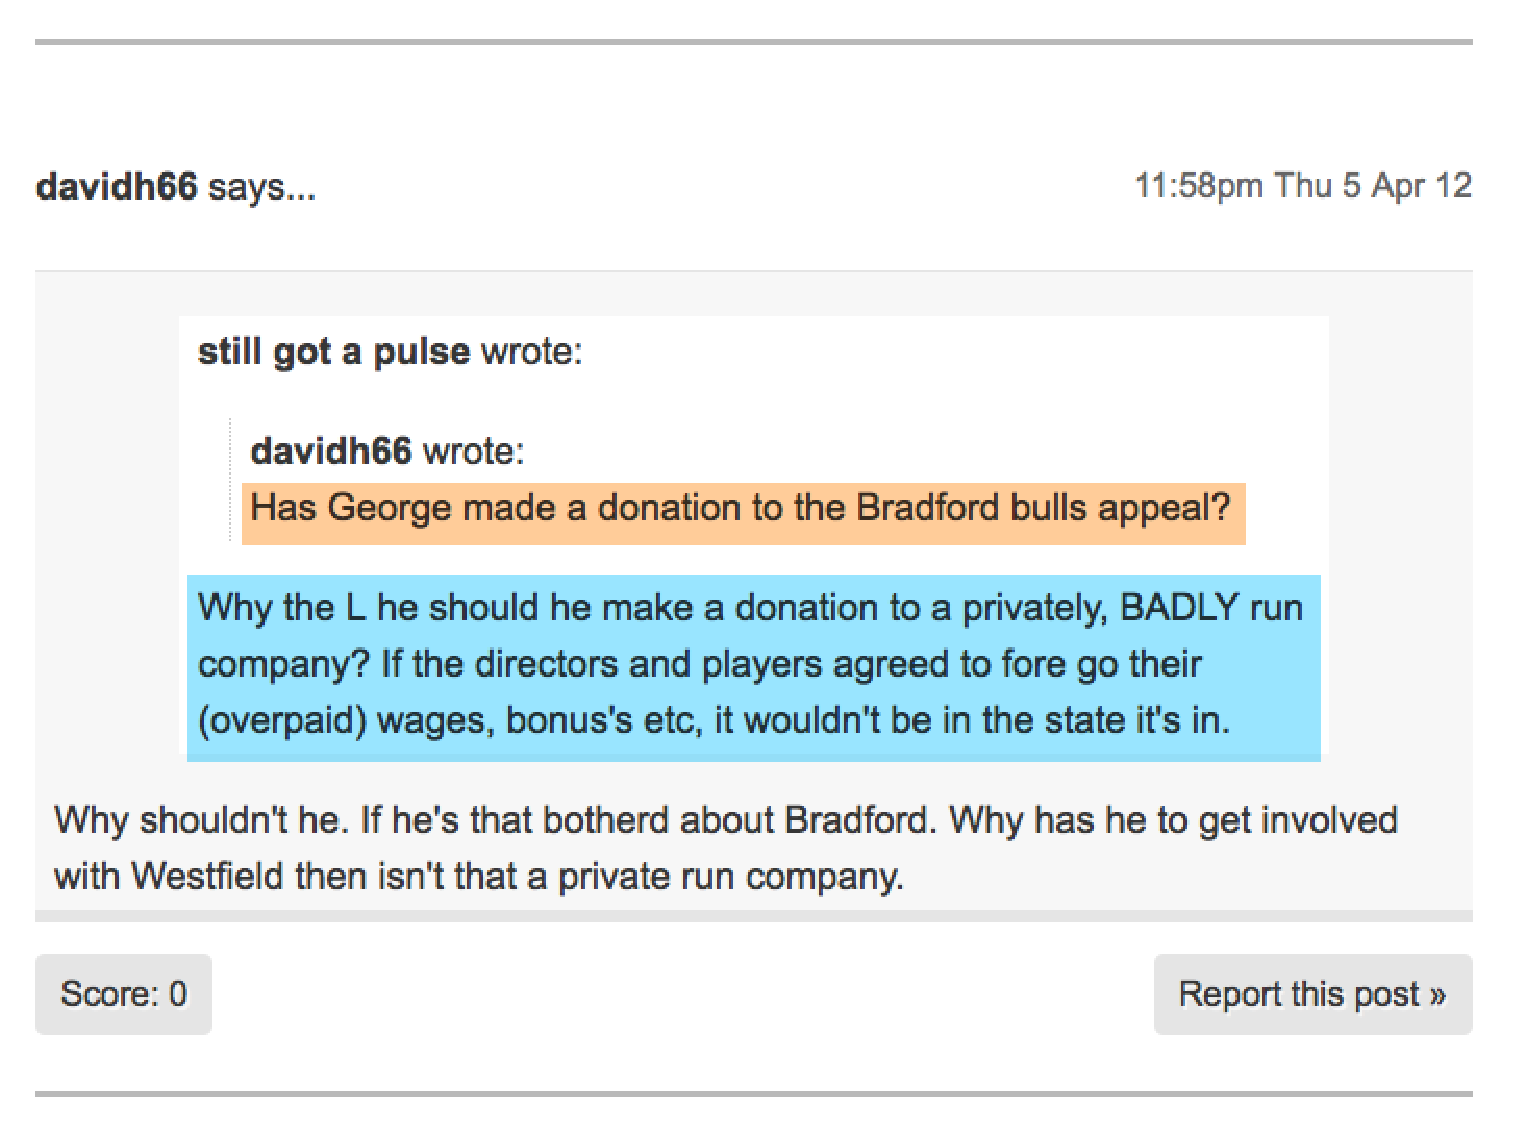
\includegraphics[width=8cm]{graphicswcc/george3col2}\\
   \end{center}
 \end{frame}


 \begin{frame}
   
  \begin{center}
     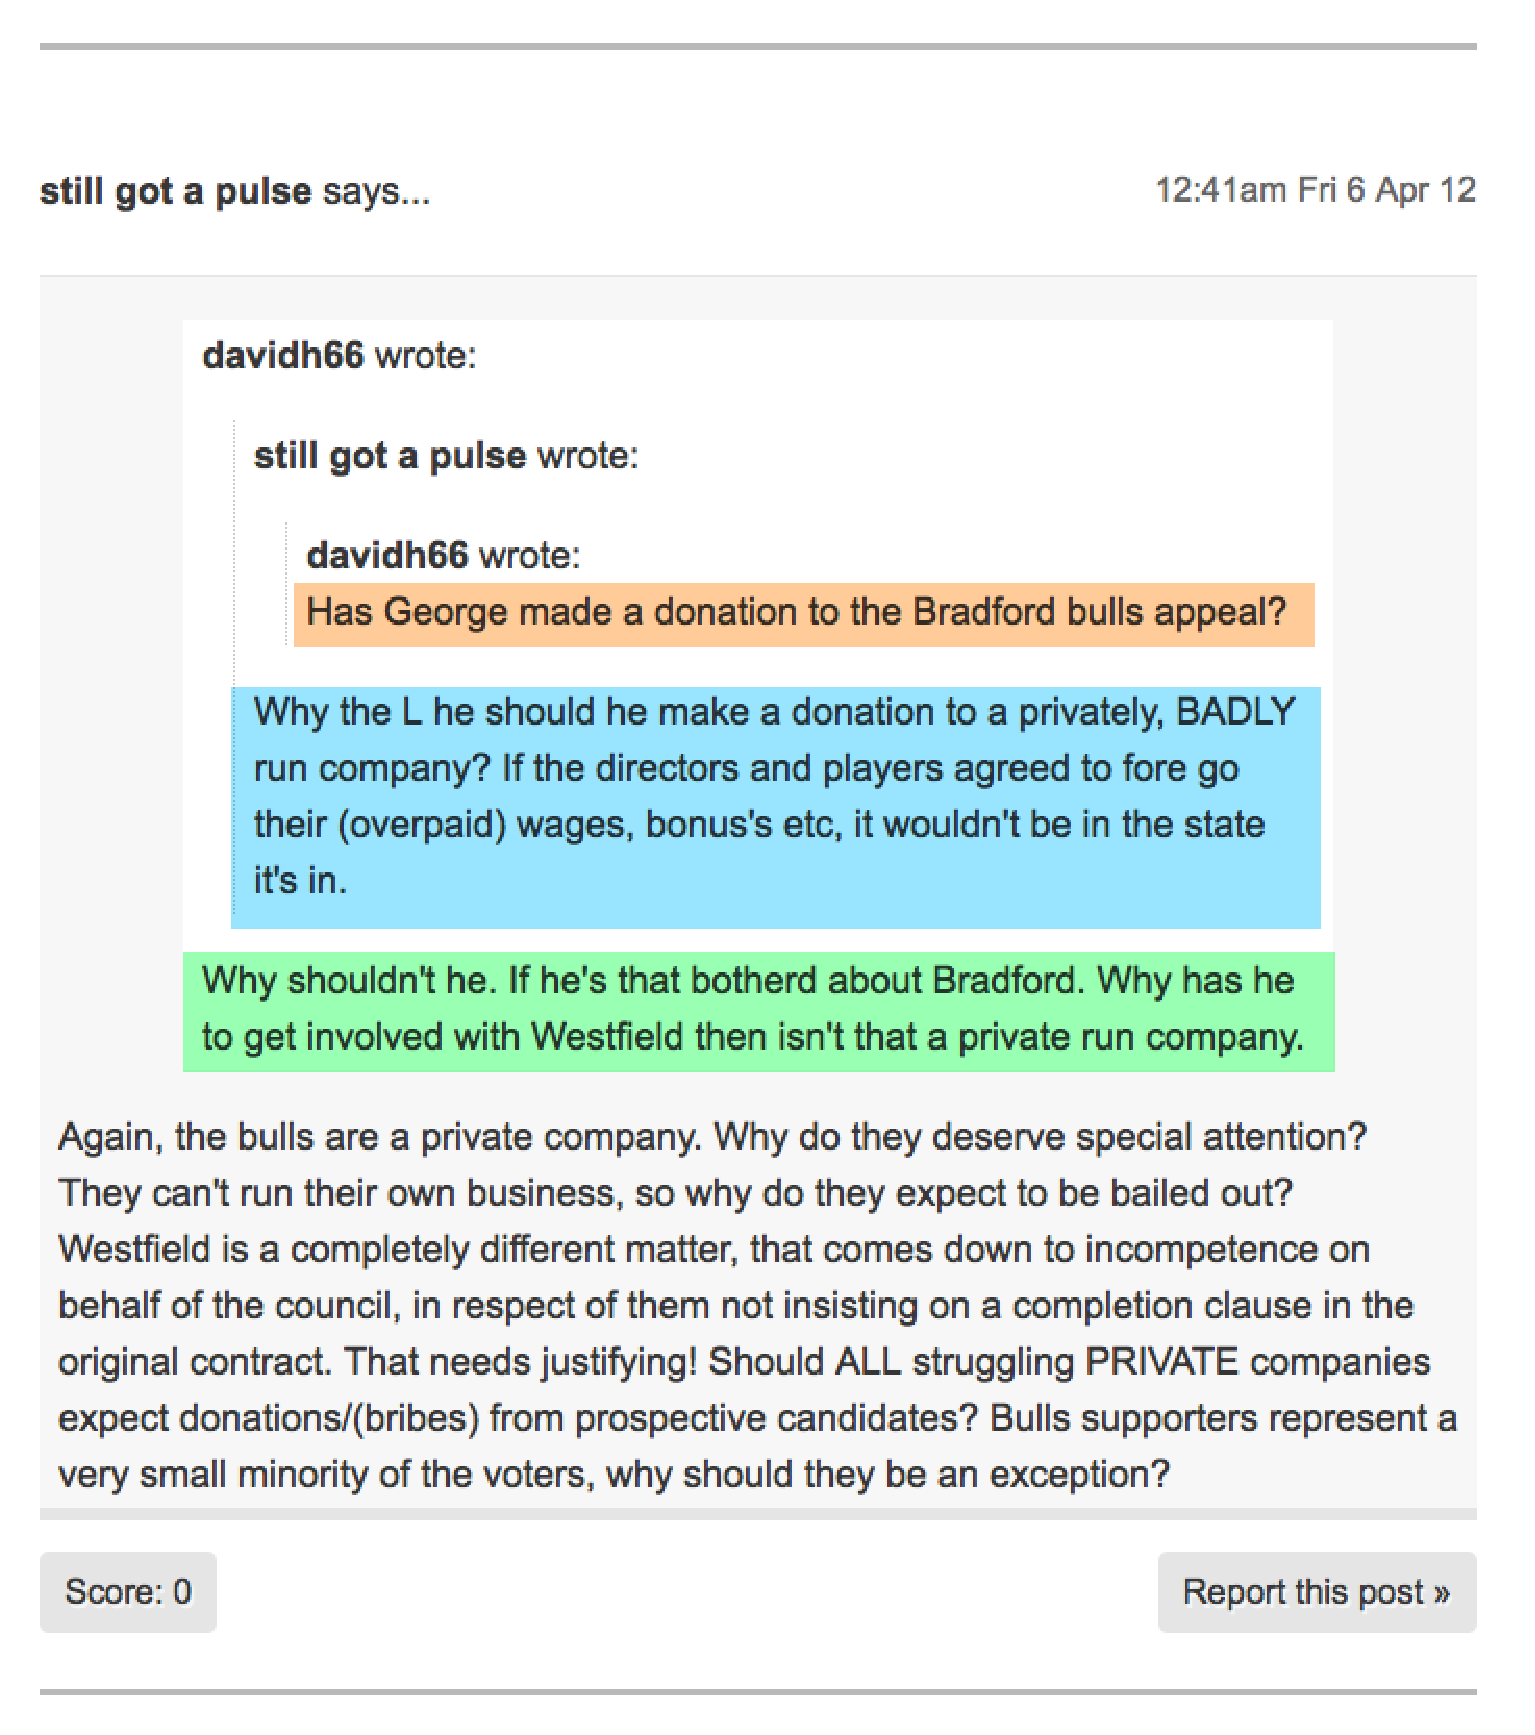
\includegraphics[width=8cm]{graphicswcc/george4col}\\
   \end{center}

 \end{frame}



\begin{frame}
  {Near duplication and inclusion}
  \begin{itemize}
    \item Many web pages are not perfect duplicates of others,\\
      but just \alert{very similar}.
    \item One typical source: slightly edited texts from news agencies\\
      in several newspapers.
    \item Also, some web pages fully contain other web pages (\alert{inclusion}).
    \item Inclusion situation is made worse by typical blog and content management systems.
  \end{itemize}
\end{frame}


% \begin{frame}
%   This is part of a month view of a blog with many postings:
%   \begin{center}
%     \includegraphics[width=8cm]{graphicswcc/lawblog}\\
%     (\url{http://www.lawblog.de/}, 11.10.2011)
%   \end{center}
% \end{frame}

% \begin{frame}
%   But each posting is also available as a single page:
%   \begin{center}
%     \includegraphics[width=8cm]{graphicswcc/lawblog_einzeln}\\
%     {\scriptsize(\url{http://www.lawblog.de/index.php/archives/2011/10/07/erotische-schriften/})}
%   \end{center}
% \end{frame}

%\begin{frame}
%  {Failure of perfect duplicate hashing/fingerprinting}
%  \begin{center}
%    $D_1$ : \alert<3>{Y}esterday\alert<4>{,} I wrote a le\alert<5>{t}ter to my pa\alert<6>{r}ents.\\
%    $D_2$ : \alert<7>{Y}esterday \alert<7>{I} wrote a let\alert<7>{t}er to my par\alert<7>{e}nts.
%  \end{center}
%  \begin{itemize}
%    \item<2> Hashes (\eg, SHA1 -- very, maybe too strong for the given task):
%      \begin{itemize}
%	\item 12d952c23cc3869faead1e1aa6e02b98256e35f8
%	\item 5ad8468fcb45fe07ef420fd87cd360087514d1f1
%      \end{itemize}
%  %  \item <3->Fingerprints using every tenth character:
%  %    \begin{itemize}
%%	\item<3-> $D_1$: \alert<3>{y}\alert<4>{,}\alert<5>{t}\alert<6>{r}
%%	\item<7-> $D_2$: \alert<7>{y}\alert<7>{i}\alert<7>{t}\alert<7>{e}
% %     \end{itemize}
%  \end{itemize}
%\end{frame}
%
%
%%\subsection{Jaccard Coefficients}
%\begin{frame}
%  {Solution -- in principle: Jaccard Coefficients}
%  \begin{itemize}
%    \item One can measure the similarity of two documents as \\
%      \alert{the Jaccard Coefficient of the sets of their n-grams}\\
%      \citep[61,438]{Manning-ea2009}. 
%      \vspace{.2cm}
%    \item Procedure:
%      \begin{itemize}
%	\item Create the documents' word\slash token-n-grams.
%	\item Calculate the \alert{Jaccard Coefficient} of the two sets.
%	\item If it is above a certain threshold, delete the shorter\\
%	  of the two documents.
%      \end{itemize}
%  \end{itemize}
%\end{frame}
%
%\begin{frame}
%  {Example: High similarity with JC over token-bi-grams I}
%  \begin{center}
%    \alert<1>{Yesterday}\alert<1-2>{,} \alert<2-3>{I} \alert<3-4>{wrote} \alert<4-5>{a} \alert<5-6>{letter} \alert<6-7>{to} \alert<7-8>{my} \alert<8-9>{parents}\alert<9>{.}\\
%\vspace{.5cm}
%    $FP(D_1)=$\{\alert<1>{(yesterday;,)}, \alert<2>{(,;i)}, \alert<3>{(i,wrote)}, \alert<4>{(wrote;a)}, \alert<5>{(a;letter)}, \alert<6>{(letter;to)}, \alert<7>{(to;my)}, \alert<8>{(my;parents)}, \alert<9>{(parents;.)}\}\\
%\vspace{.5cm}
%    \onslide<10->{Yesterday I wrote a letter to my parents.\\
%\vspace{.5cm}
%    $FP(D_2)=$\{(yesterday;i), (i,wrote), (wrote;a), (a;letter), (letter;to), (to;my), (my;parents), (parents;.)\}}
%  \end{center}
%\end{frame}
%
%\begin{frame}
%  {Example: High similarity with JC over token-bi-grams II}
%  \begin{center}
%    $FP(D_1)=$\{\alert<2>{(yesterday;,)}, \alert<2>{(,;i)}, \alert<1-2>{(i,wrote)}, \alert<1-2>{(wrote;a)}, \alert<1-2>{(a;letter)}, \alert<1-2>{(letter;to)}, \alert<1-2>{(to;my)}, \alert<1-2>{(my;parents)}, \alert<1-2>{(parents;.)}\}\\
%\vspace{.5cm}
%$FP(D_2)=$\{\alert<2>{(yesterday;i)}, \alert<1-2>{(i,wrote)}, \alert<1-2>{(wrote;a)}, \alert<1-2>{(a;letter)}, \alert<1-2>{(letter;to)}, \alert<1-2>{(to;my)}, \alert<1-2>{(my;parents)}, \alert<1-2>{(parents;.)}\}\\
%\vspace{1cm}
%$J(D_1,D_2)=\frac{|D_1\cap D_2|}{|D_1\cup D_2|}=\frac{7}{10}=0.7$
%%$J(D_1,D_2)=\frac{\alert<1>{|D_1\cap D_2|}}{\alert<2>{|D_1\cup D_2|}}=\frac{\alert<1>{7}}{\alert<2>{10}}=0.7$
%  \end{center}
%\end{frame}
%
%\begin{frame}
%  {Example: Low similarity with JC over token-bi-grams}
%  \begin{center}
%    $FP(D_2)=$\{\alert{(yesterday;i)}, (i,wrote), (wrote;a), (a;letter), (letter;to), \alert{(to;my)}, (my;parents), (parents;.)\}\\
%\vspace{0.5cm}
%$D_3=$Yesterday I read a book to my niece.\\
%\vspace{0.5cm}
%$FP(D_3)=$\{\alert{(yesterday;i)}, (i,read), (read;a), (a;book), (book;to), \alert{(to;my)}, (my;niece), (niece;.)\}\\
%\vspace{1cm}
%$J(D_2,D_3)=\frac{|D_2\cap D_3|}{|D_2\cup D_3|}=\frac{2}{14}=0.14$
%  \end{center}
%\end{frame}
%
%\begin{frame}
%  {Can it be done?}
%   \begin{itemize}
%     \item 10,000,000 documents\\[1ex]
%     \item $\approx \frac{10,000,000^2}{2} = 5 \times 10^{13}$ comparisons\\[1ex]
%     \item at $1\mu s$ per comparison: $\approx$ 579 days
%     \item \graw{But $1\mu s$ is faster than available processors can do it.}
%   \end{itemize}
%
%\pause
%
%Solution:  
%
%
%\begin{itemize}
%\item Do not \textbf{calculate} JC for each pair of documents.
%\item Instead, \textbf{estimate} the JC \citep{Broder-ea1997}.
%\item Technique is known as \textit{w-Shingling}.
%\end{itemize}
%
%\end{frame}
%
%
%



 \begin{frame}
{Near-duplicate detection with \texttt{w-shingling}}

\texttt{w-shingling} does not tell us which amount of duplication\\
is acceptable in a corpus.

\begin{itemize}
 \item<1-> Setting a particular JC as a threshold for keeping/discarding\\
   a document is ultimately an arbitrary choice
    \begin{itemize}
    \item Design decision by corpus builders. 
    \end{itemize}
\item<2-> Web corpora will probably always contain a certain amount\\
  of duplication
    \begin{itemize}
    \item many other corpora do, too
    \end{itemize}

\item<3-> Strategies to cope with duplication:
   \begin{itemize}
   \item If compatible with research question:\\
     work with sentence-wise uniq'ed corpora.
   \item Or work with unique (not too short) concordance lines.
   \end{itemize}


\end{itemize}
 
 \end{frame}


\subsection{Linguistic post-processing}


\begin{frame}
  {Noise in web corpora: sources}

  \begin{enumerate}
 \item <1-> properties of web-documents, e.\,g.
    \begin{itemize}
    \item quasi-spontaneous writing situations with (often)\\
      casual language, typos, non-standard spellings,\\
      improper use of whitespace and punctuation
    \item text contributed by non-native speakers 
    \item a large lexicon with many out-of-vocabulary items
   \end{itemize}
  \item<2-> the structure of the WWW and its technologies, e.\,g.
    \begin{itemize}
    \item duplicated text, boilerplate
    \end{itemize}
  \item<2-> shortcomings in post-processing, e.\,g.
    \begin{itemize}
    \item HTML/code-stripping, tokenization 
    \end{itemize}
  \end{enumerate}
\end{frame}



% \begin{frame}{Example: spelling variants}
  
% \begin{figure}[h]
%   \centering
%   \scalebox{.7}{
%     \begin{tabular}{lc@{\hspaceThis{XXXXXXXXXXX}}lrr}
%       Correct form (frequency)& & Misspelled form & N & edit distance \\
%       \hline
%       &&\node{a}{\alert{u}bernimmt} & 81 & 1 \\
%       &&\node{b}{überni\alert{n}mmt}& 6 & 1\\
%       &&\node{c}{übernimm\alert{n}t}& 1 & 1\\
%       &&\node{d}{überni\alert{e}mt} & 6 & 1\\
%       &&\node{e}{\alert{ö}bernimmt} & 6 & 1\\
%       &&\node{f}{übernim\alert{n}mt}& 5 & 1\\
%       &&\node{h}{übernimm\alert{e}t}& 11 & 1\\
%       \node{x}{übernimmt (297440)}&&\node{i}{überni\alert{eh}mt} & 2 & 2\\
%       &&\node{j}{überni\alert{e}mt} & 6 & 1\\
%       &&\node{k}{überni\alert{h}mt} & 17 & 1\\
%       &&\node{l}{überni\alert{iiiiiiimmmmm}mmt} & 1 & 12\\
%       &&\node{m}{überni\alert{o}mmt}& 4 & 1\\
%       &&\node{n}{übernim\alert{rn}t}& 4 & 2\\
%       &&\node{p}{überni\alert{u}mmt}& 2 & 1\\
%       &&\node{q}{überni\alert{nn}t} & 2 & 2\\
%       &&\node{r}{übernimm\alert{t}t}& 2 & 1\\
%       &&\node{o}{\ldots}
%     \end{tabular}
% %    \anodeconnect[r]{x}[l]{a}
% %    \anodeconnect[r]{x}[l]{b}
% %    \anodeconnect[r]{x}[l]{c}
% %    \anodeconnect[r]{x}[l]{d}
% %    \anodeconnect[r]{x}[l]{e}
% %    \anodeconnect[r]{x}[l]{f}
% %    \anodeconnect[r]{x}[l]{h}
% %    \anodeconnect[r]{x}[l]{i}
% %    \anodeconnect[r]{x}[l]{j}
% %    \anodeconnect[r]{x}[l]{k}
% %    \anodeconnect[r]{x}[l]{l}
% %    \anodeconnect[r]{x}[l]{m}
% %    \anodeconnect[r]{x}[l]{n}
% %    \anodeconnect[r]{x}[l]{p}
% %    \anodeconnect[r]{x}[l]{q}
% %    \anodeconnect[r]{x}[l]{r}
% %    \anodeconnect[r]{x}[l]{o}
%   }



% \end{figure}

% \end{frame}


\begin{frame}{Example: text produced by non-native speakers}
\begin{center}
     \includegraphics[width=11cm]{graphicswcc/walkman}\\
   \end{center}
\end{frame}



\begin{frame}
{Noise in linguistic post-processing}

Most available natural language processing tools expect standard written language as input.

\begin{itemize}
\item Many tokenizers expect proper use of whitespace,\\
  casing and punctuation.
\item Part-of-speech taggers expect properly tokenized text as input.
\item POS-taggers usually perform worse on unknown items\\
     (tokenization errors, misspellings, out-of-vocabulary items).
\item Proper tokenization and POS tagging is normally the basis\\
  for higher-level linguistic annotation\\
  (parsing, sense disambiguation etc.).
\end{itemize}
\end{frame}



\begin{frame}
{Should noise be ``normalized away''?}

What exactly is ``noise'' in the first place?

\begin{itemize}
\item No general definition of ``noise'' that suits all purposes
\item What counts as noise in one task may be valuable data\\
  in another task
\end{itemize}
\end{frame}


\begin{frame}
{Can noise be ``normalized away''?}


In large web corpora, noise would have to be eliminated automatically, without human interaction.\\[1ex]

\begin{itemize}
\item viable in some cases:
  \begin{itemize}
  \item e.\,g.\ correcting run-together words\\
   \texttt{a \alert{lot.I} don't think} $\rightarrow$\  \texttt{a lot. I don't think} 
  \end{itemize}
\vspace{1cm}
\pause
\item but not an easy task in other cases:
  \begin{itemize}
  \item e.\,g.\ spelling correction\\
   \texttt{I didn't spend much time with \alert{Bibble}.} $\rightarrow$ \textit{Bubble}?
  \end{itemize}
\end{itemize}
\end{frame}



%\begin{frame}
%  {Non-destructive normalization}
%Our approach: do as much as possible non-destructively\\
%(i.\,e.\, do not alter the original data).
%\begin{itemize}
%\item Normalization-as-annotation
%\item But there are limits to this approach imposed\\
%  by the indexing/query architecture.
%\end{itemize}
%\end{frame}
%
%
%\begin{frame}{Non-destructive orthographic normalization}
%
%\setlength{\columnsep}{1cm}
%\begin{multicols}{2}
%  \scalebox{.8}{
%   \ttfamily
%    \begin{tabular}{llll}
%      & \textbf{Word} & \textbf{POS} & \textbf{Lemma} \\
%      \cline{2-4}
%      & The     & DT    & the   \\
%      & FA      & NP    & FA    \\
%      & does    & VBZ   & do    \\
%      & \alert{abosolutley}&\alert{JJ}&\alert{$<$unknown$>$}\\
%      & nothing & NN    & nothing       \\
%      & to      & TO    & to    \\
%      & help    & VB    & help  \\
%      & Clubs   & NNS   & club  \\
%    \end{tabular}
%  }
%
%\columnbreak
%\onslide<2->{
% \scalebox{.8}{
%    \ttfamily
%    \begin{tabular}{llll}
%      & \textbf{Word} & \textbf{POS} & \textbf{Lemma} \\
%      \cline{2-4}
%      & The     & DT    & the   \\
%      & FA      & NP    & FA    \\
%      & does    & VBZ   & do    \\[0.8ex]
%      \multicolumn{4}{l}{$<$norm from="{}abosolutley"$>$} \\[0.8ex]
%      & \alert{absolutely} &\alert{ADV}&\alert{absolutely} \\[0.8ex]
%      \multicolumn{4}{l}{$<$/norm$>$} \\[0.8ex]
%      & nothing & NN    & nothing       \\
%      & to      & TO    & to    \\
%      & help    & VB    & help  \\
%      & Clubs   & NNS   & club  \\
%    \end{tabular}
%  }
%}
%\end{multicols}
%
%%\vspace{.2cm}
%
%\begin{multicols}{2}
%{\footnotesize
%Original text: spelling error, POS-tagging error, no lemma
%
%\columnbreak
%\onslide<2->{
%Normalized text: standard spelling, correct POS and lemma, original spelling preserved as meta data
%}
%}
%\end{multicols}
%
%\end{frame}


\begin{frame}
  {Quality of linguistic annotation in web corpora}

Automatic annotation may be concern, e.\,g.\

\begin{itemize}
\item Do not take type counts in web corpora at face value.
  \begin{itemize}
  \item There are many \textit{hapax legomena} due to tokenization issues.
  \end{itemize}
\item POS tagging of web corpora does not quite reach\\
  accuracy levels in the upper 90\%
  \begin{itemize}
  \item but many POS taggers do not reach such accuracy levels\\
    on traditional, out-of-domain texts either
  \end{itemize}
\end{itemize}

\pause

But:

\begin{itemize}
\item Depending on the specific research question,\\
  some or all of these problems by irrelevant.
\item Anyway, in many scenarios, there is no alternative\\
  to working with web corpora.
\item \alert{And do not expect the situation to be perfect with other corpora!}
\end{itemize}

\end{frame}



